\documentclass{article}
\usepackage[utf8]{inputenc}
\usepackage[T1]{fontenc}
\usepackage{lmodern}
\usepackage[margin=2.5cm]{geometry}
\usepackage{amsfonts}
\usepackage{amsmath}
\usepackage{bbm}
\usepackage{amsthm}
\usepackage{blkarray}
\usepackage{amsmath}
\newtheorem{lemma}{Lemma}
\newtheorem{corollary}{Corollary}
\usepackage{soul}
\usepackage[export]{adjustbox}
\usepackage[footnotes,definitionLists,hashEnumerators,smartEllipses, hybrid]{markdown}

\usepackage[usenames, dvipsnames]{color}
\usepackage{lmodern}
\definecolor{gray}{rgb}{0.5, 0.5, 0.5}
\newcommand{\RPack}[1]{\textsf{#1}}
\newcommand{\RCmd}[1]{\texttt{#1}}
\newcommand{\RObj}[1]{\texttt{#1}}
\newcommand{\soft}[1]{\texttt{#1}}

\newcommand{\sd}[1]{\textcolor{magenta}{*** SD: #1}}
\newcommand{\fp}[1]{\textcolor{blue}{*** FP: #1}}
\newcommand{\dr}[1]{\textcolor{red}{*** DR: #1}}
\newcommand{\ks}[1]{\textcolor{green}{*** KS: #1}}


\usepackage{authblk}

\usepackage[backend=biber]{biblatex}
\addbibresource{Mendeley_zinbsurf.bib}
\IfFileExists{upquote.sty}{\usepackage{upquote}}{}

\makeatletter
\g@addto@macro\appendix{\renewcommand{\thefigure}{S\arabic{figure}}\setcounter{figure}{0}}
\makeatother

\usepackage[colorlinks=true,linkcolor=black,anchorcolor=black,citecolor=black,filecolor=black,menucolor=black,runcolor=black,urlcolor=black]{hyperref}

\newcommand*\samethanks[1][\value{footnote}]{\footnotemark[#1]}
\usepackage[colorlinks=true,linkcolor=black,anchorcolor=black,citecolor=black,filecolor=black,menucolor=black,runcolor=black,urlcolor=black]{hyperref}

\title{Using ZINB-WaVE within the zingeR framework to unlock RNA-seq tools for scRNA-seq}
\author{Fanny Perraudeau, Davide Risso, Jean-Philippe Vert, Sandrine Dudoit}

\date{\today}
\begin{document}
\maketitle

\bigskip

This work was inspired by the zingeR approach described in the preprint \cite{VandenBerge2017ZingeR:Applications}.

\section*{Introduction}

\section*{Results}

\subsection*{ZINB-WaVE unlocks bulk RNA-seq DE tools for scRNA-seq by handling zero inflation}

In \cite{Risso2017}, we proposed Zero-Inflated Negative Binomial-based Wanted Variation Extraction (ZINB-WaVE), a general and flexible method that uses a zero-inflated negative binomial (ZINB) model to extract low-dimensional signal from scRNA-seq read counts, accounting for zero inflation (dropouts), over-dispersion, and the discrete nature of the data. According to the ZINB-WaVE model, the posterior probability of belonging to the negative binomial (NB) count component for cell $i$ and gene $j$ can be computed as follows
\begin{equation}W_{ij} = \frac{ ( 1 - \pi_{ij} ) f_{NB}(y_{ij}; \mu_{ij}, \theta_j ) }{f_{ZINB}(y_{ij};\mu_{ij}, \theta_j, \pi_{ij})},
\end{equation}
where $y_{ij}$ denotes the read count for gene $j$ in cell $i$ and $f_{NB}(\cdot; \mu, \theta)$ and $f_{ZINB}(\cdot; \mu, \theta, \pi)$ denote, respectively, the NB and ZINB probability mass functions with mean $\mu$, dispersion $\theta$, and dropout probability $\pi$ (see Methods section for notation and details about the model). As in \cite{VandenBerge2017ZingeR:Applications}, the posterior probabilities $W_{ij}$ can be used as observation-level weights in tools for bulk RNA-seq differential expression (DE) analysis such as edgeR, DESeq2, or limma-voom.\\ 

The observation-level weights estimated using ZINB-WaVE differ from those estimated using zingeR in the following important respects. First of all, while the zingeR model uses a constant (across all genes) probability $\pi_i$ of dropout for each cell $i$, the probability of dropout $\pi_{ij}$ for ZINB-WaVE is both cell and gene-specific. The latter approach, adopted in recent methods \cite{Pierson2015ZIFA:Analysis} \cite{Finak2015MAST:Data}, is likely to result in a better fit to the data. Secondly, the ZINB-WaVE negative binomial mean $\mu$ and zero inflation probability $\pi$ are modeled in terms of both wanted and unwanted cell and gene-level covariates, allowing normalization for a variety of nuisance technical effects. Thirdly, parameters of the zingeR and ZINB-WaVE models are estimated using different methods: parameters from the zingeR model are estimated using the EM algorithm, whereas those from the ZINB-WaVE model are estimated using a penalized likelihood method.

\subsection*{ZINB-WaVE yields high power and low Type I error rate on simulated data}

\subsubsection*{High sensitivity and specificity}
Messages:
\begin{enumerate}
\item best method is zinbwave-edgeR followed by zinbwave-DESeq2. zingeR-edgeR and zingeR-DESeq2 performs ok. zingeR-limmavoom or zinbwave-limmavoom performs poorly. Maybe weights not use the correct way for limma. Other methods perform poorly. See Figure \ref{f:islamFC2} for fold change 2 and same figure for fold change 3 (to come in suppl.). See Figure\ref{f:islamTableFC2}.
\item zingeR and zinbwave might have different results because of different estimation of the parameters. For example, probability to observe a zero instead of actual count is $\pi_i$ in zingeR but $\pi_{ij}$ in ZINB-WaVE. It results in difference of weights (Figure \ref{f:islamWeightsFC2}) and dispersion (Figure \ref{f:islamDispFC2})
\item no big difference between genewise and common dispersion. See Figures \ref{f:islamFC2zinbwave}. Could be explained by no big diff in weights (see Figure \ref{f:qqplotFC2}) and disp. (see Figure \ref{f:islamDispFC2}). Genewise dispersion is 15 times slower than common. We think that common dispersion is a good approximation. 
\end{enumerate}

\subsubsection*{Controlled FDR at 0.05}
Messages:
\begin{enumerate}
\item FDR is controlled by zingeR and zinbwave but not by MAST. See Figure \ref{f:mocks}.
\item Influence of epsilon on FPR and distribution pvalues.
\end{enumerate}

\subsection*{ZINB-WaVE leads to biologically meaningful DE genes}
Fletcher dataset

\section*{Discussion}
Makes lot of sense to use tools already developed and tested.\\

We are working on using ZINB-WaVE model itself to identify differentially expressed genes, both in terms of the negative binomial mean and the zero inflation probability, reflecting, respectively, gradual DE and on/off DE patterns. (cite DEsingle) However, it is challenging. We envision two approaches: likelihood ratio test (LRT) or Wald test. Both are computationally challenging. LRT: need to refit for each hypothesis. Wald test: need to compute the Hessian matrix which is huge (dim.) and requires lots of computation. We could make assumptions but they would need to be tested. In addition, we could use ZINB-WaVE model to perform imputation.\\

\section*{Conclusions}
Better results than current methods, even the methods developped for scRNA-seq relying on state-of-the-art methods that have been developed and tested on bulk RNA-seq data.

\section*{Figures}

\begin{figure}[ht]
\begin{center}
\begin{tabular}{cccc}
\textbf{A} &
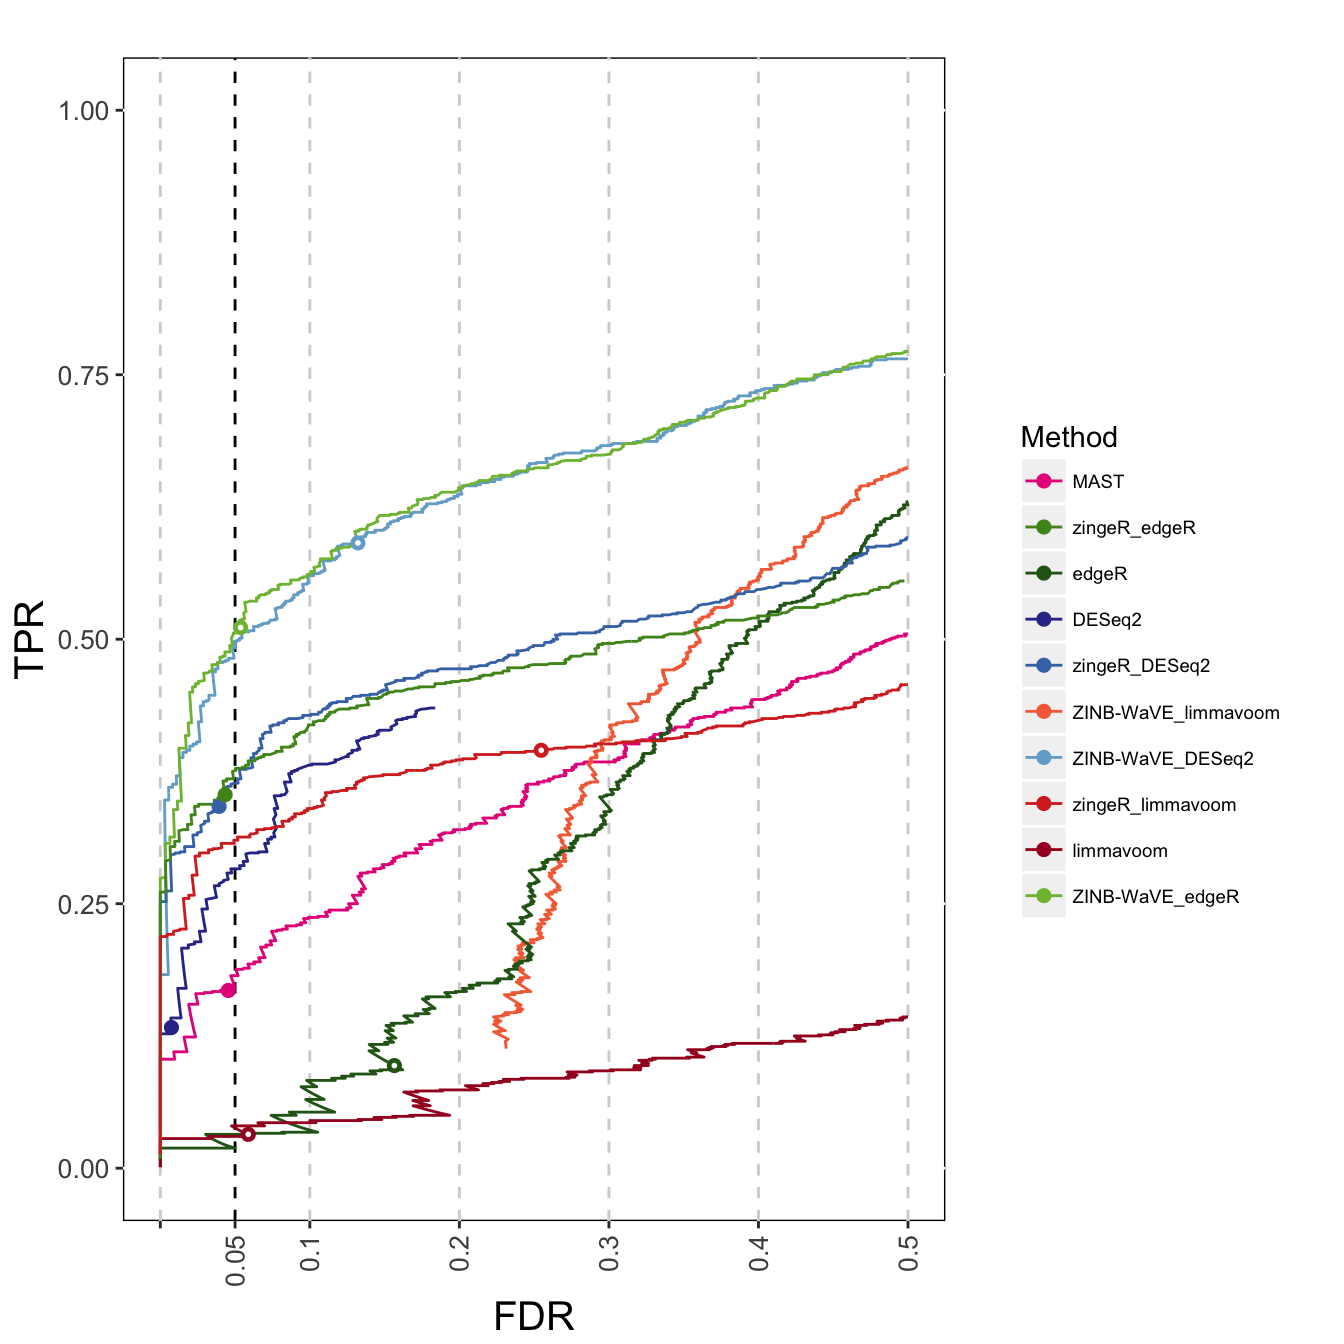
\includegraphics[keepaspectratio=true,scale=0.16,valign=t]{islamROCfc2-1} &
\textbf{B} &
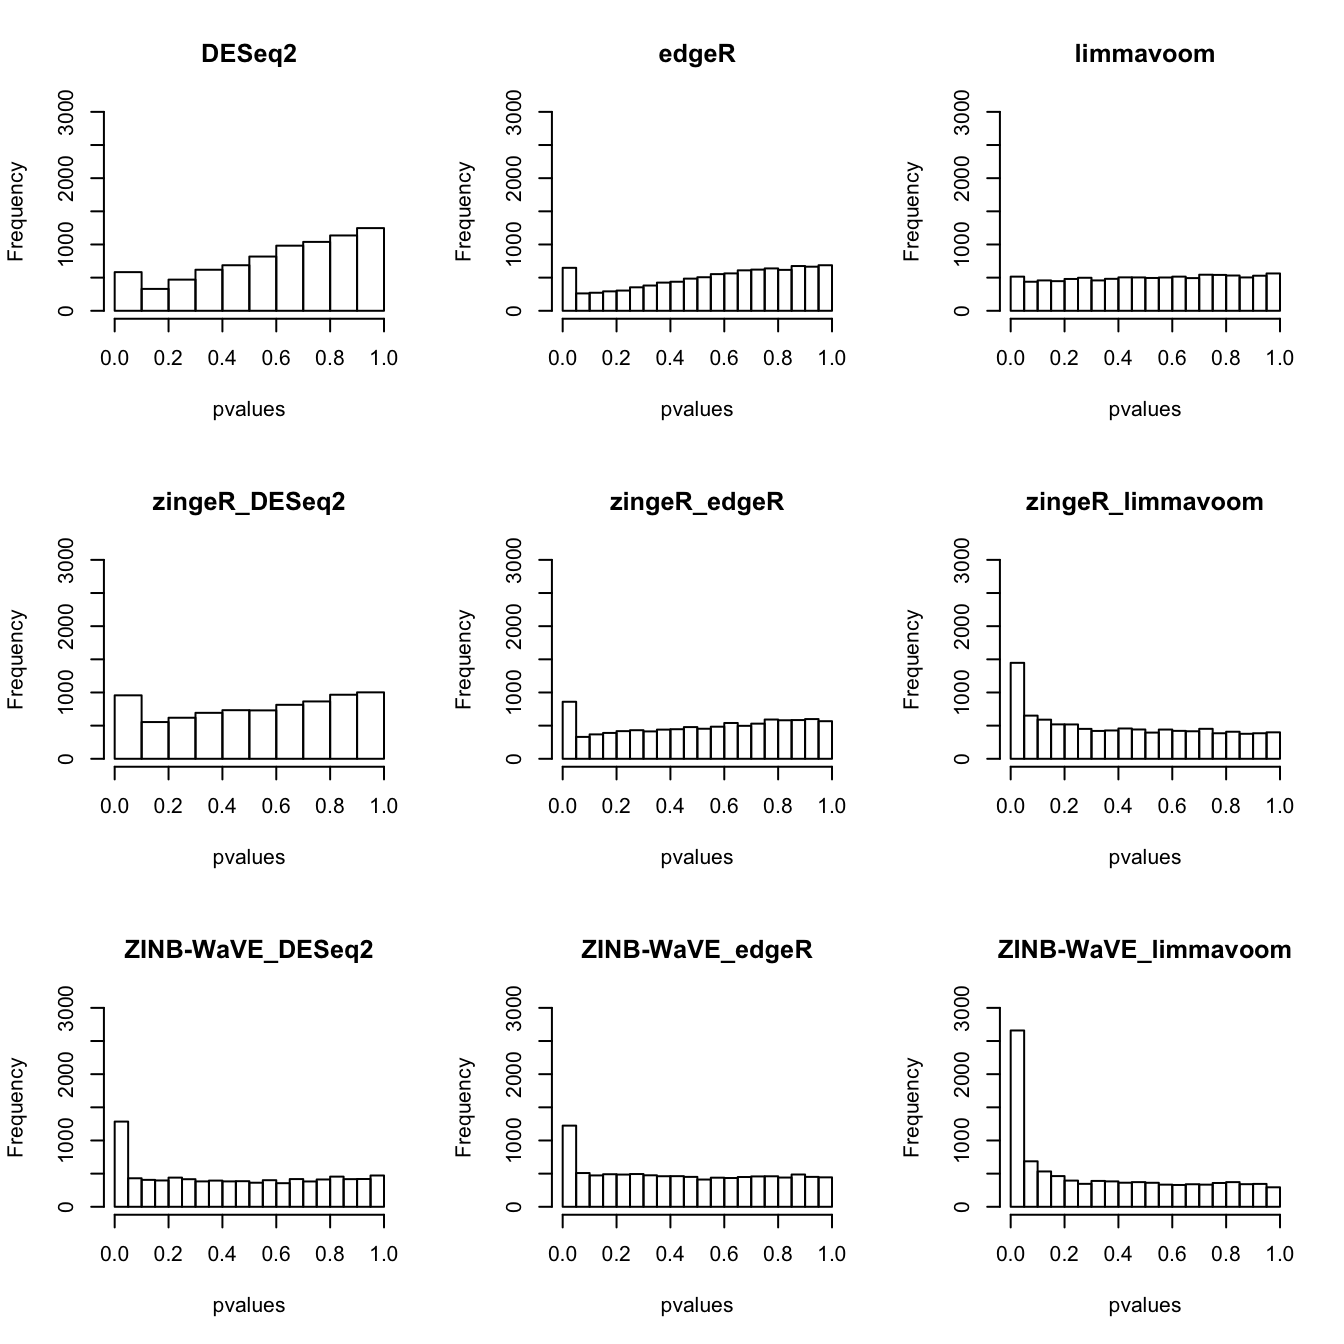
\includegraphics[keepaspectratio=true,scale=0.16,valign=t]{islamPvaluesFC2-1} 
\end{tabular}
\end{center}
\caption{{\em Simulations from Islam dataset using zingeR simulation framework.} Fold change = 2, 80 cells, 10k genes. Panel (A) : ROC. Panel (B) Distr. of pval.}
\label{f:islamFC2}
\end{figure}

\begin{figure}[ht]
\begin{center}
\begin{tabular}{cccc}
\textbf{A} &
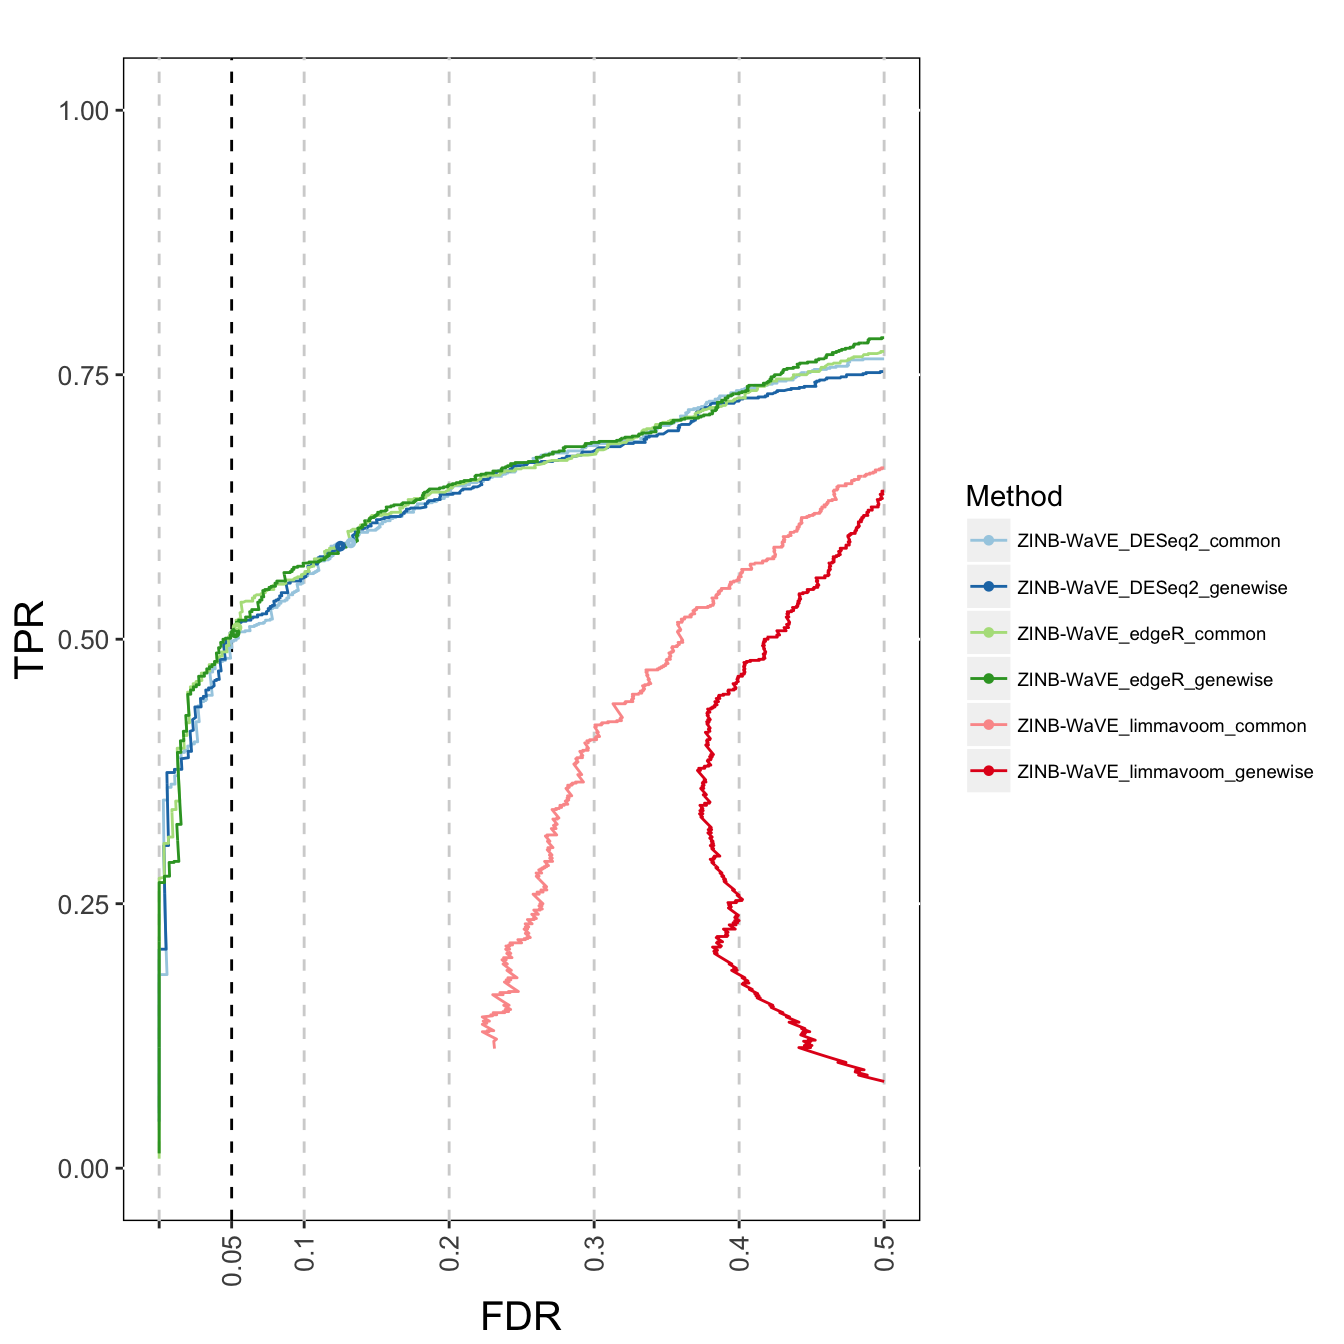
\includegraphics[keepaspectratio=true,scale=0.16,valign=t]{islamROCfc2zinbwave-1} &
\textbf{B} &
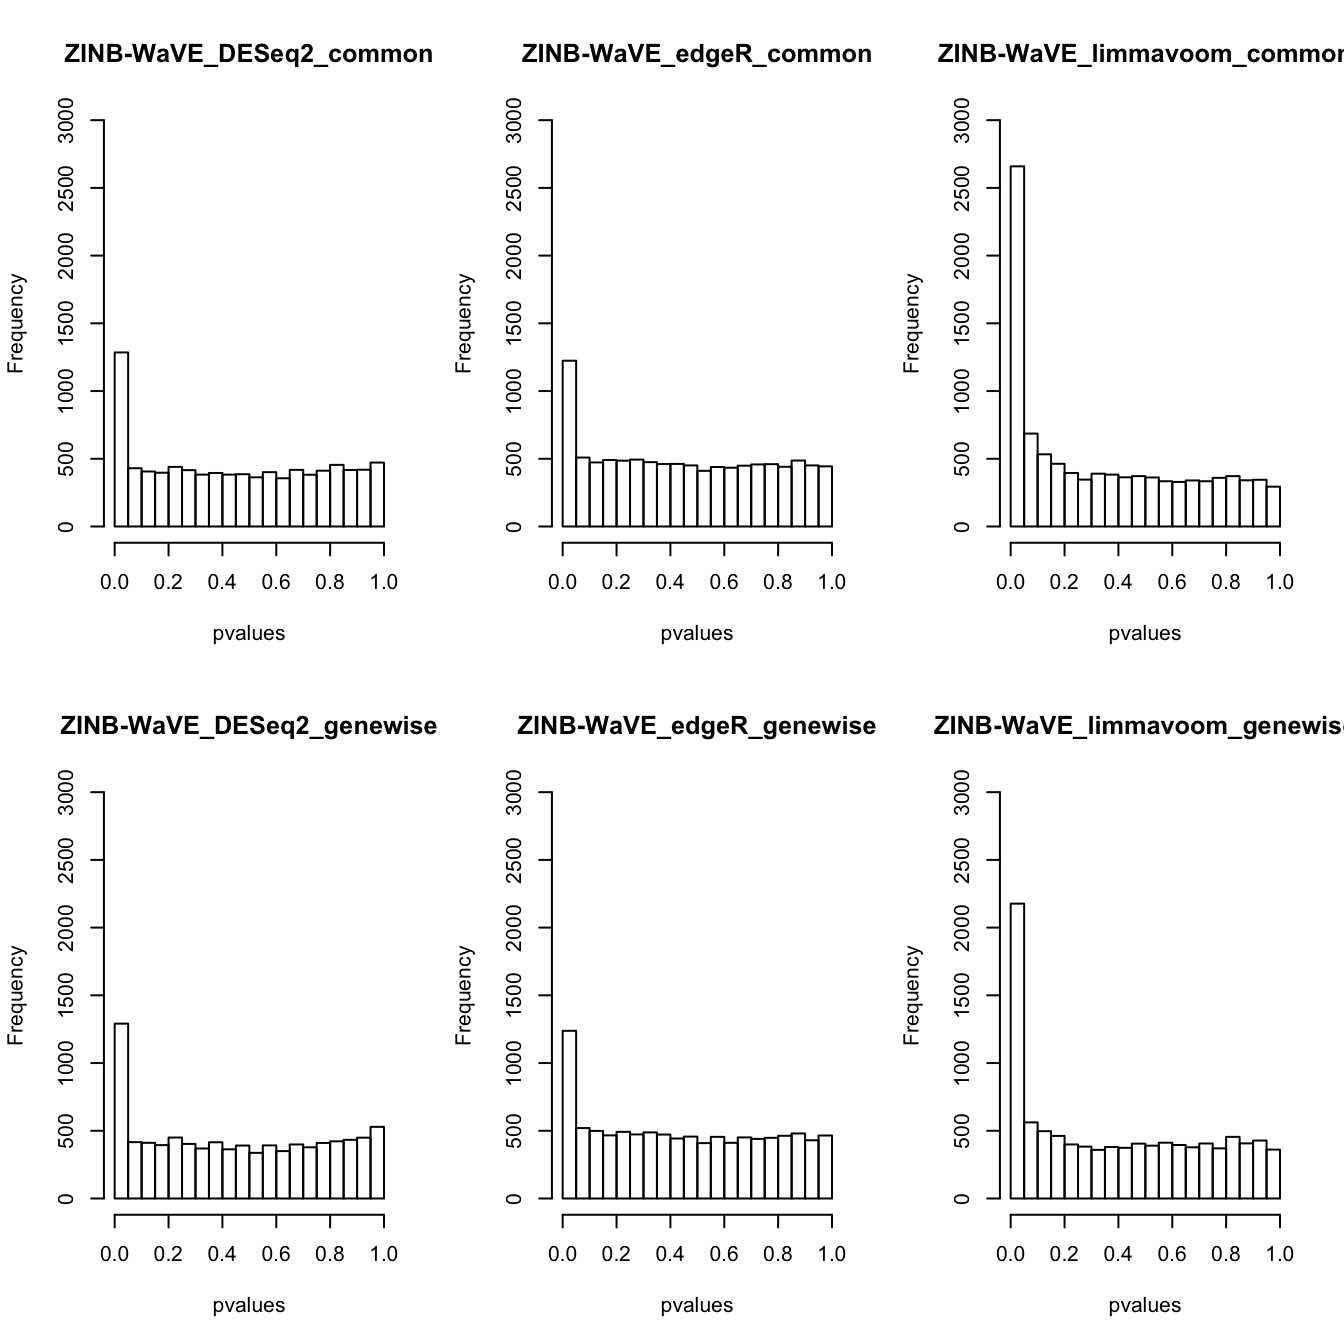
\includegraphics[keepaspectratio=true,scale=0.16,valign=t]{islamPvaluesFC2zinbwave-1} 
\end{tabular}
\end{center}
\caption{{\em Simulations from Islam dataset using zingeR simulation framework.} Compare genewise and common dispersion for ZINB-WaVE. Fold change = 2, 80 cells, 10k genes. Panel (A) : ROC. Panel (B) Distr. of pval.}
\label{f:islamFC2zinbwave}
\end{figure}


\begin{figure}[ht]
\begin{center}
\includegraphics[keepaspectratio=true,scale=0.5]{islamTableFC2}
\end{center}
\caption{{\em Table of number of DE genes, TPR, and FPR at Benjamini and Hochberg \cite{BenjaminiHochberg} adjusted $p$-value = 0.05}}
\label{f:islamTableFC2}
\end{figure}

\begin{figure}[ht]
\begin{center}
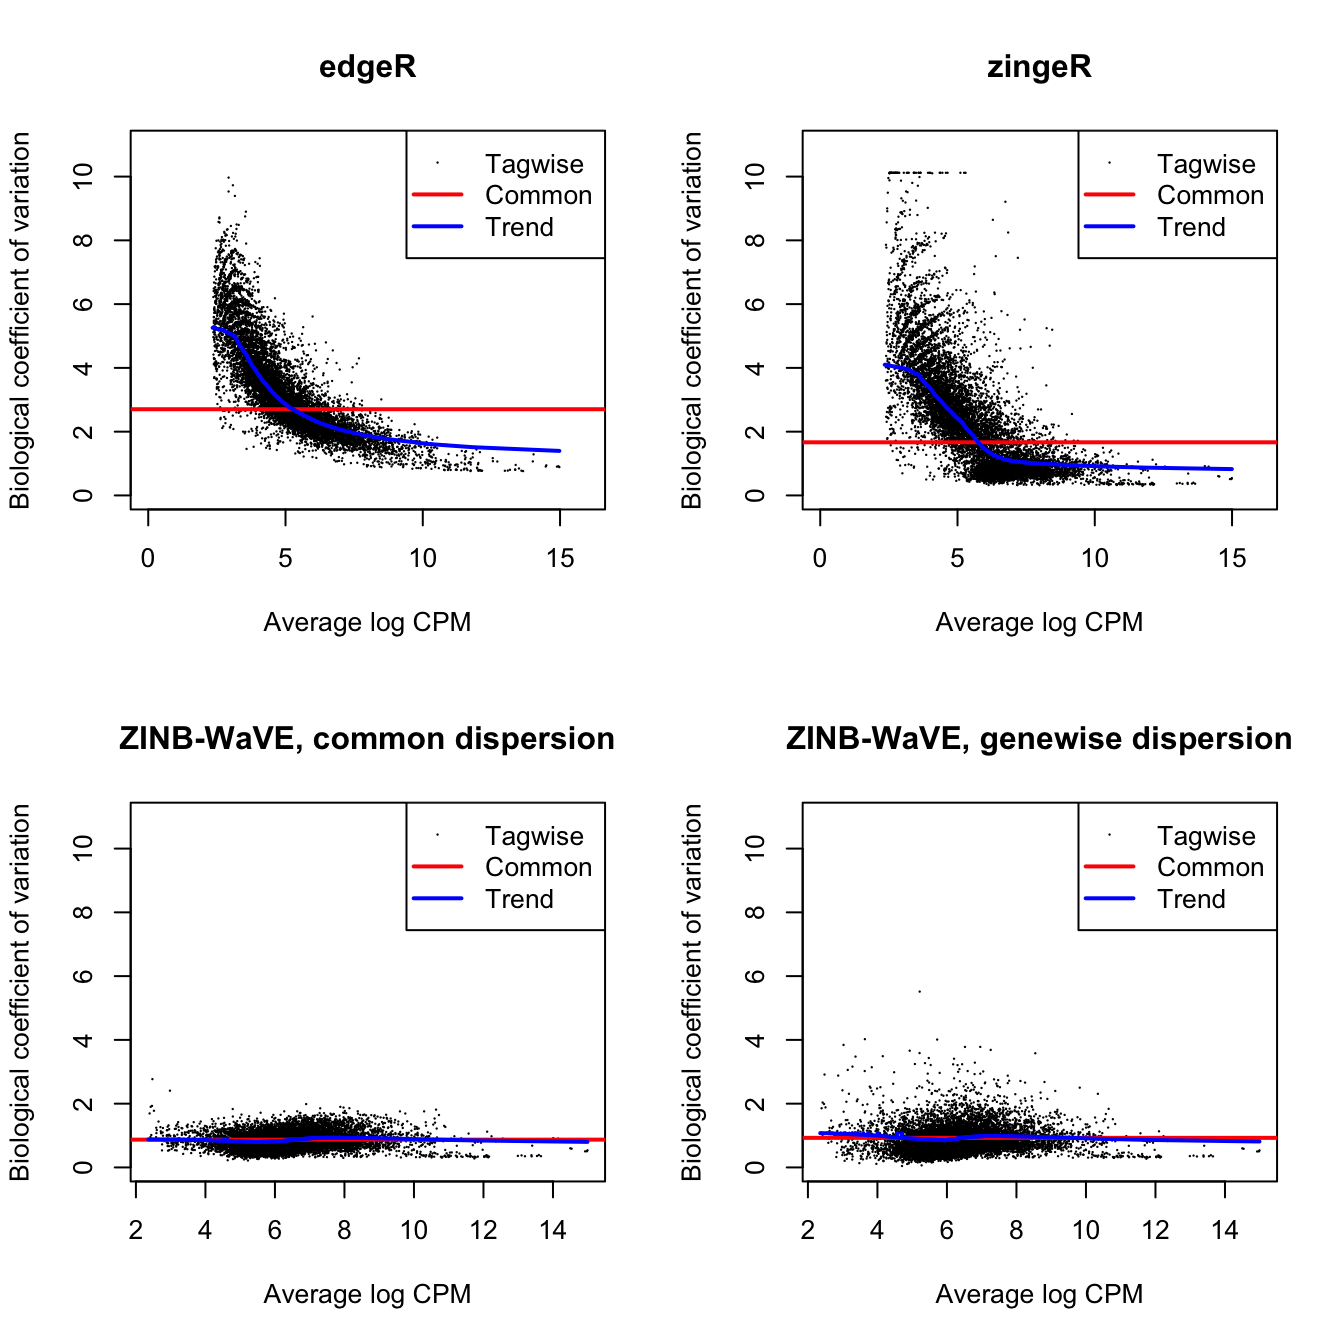
\includegraphics[keepaspectratio=true,scale=0.3]{islamDispFC2-1}
\end{center}
\caption{{\em Comparison of the biological coefficient of variation (BCV) against the average log CPM for zingeR (left) and zinbwave (right).}}
\label{f:islamDispFC2}
\end{figure}

\begin{figure}[ht]
\begin{center}
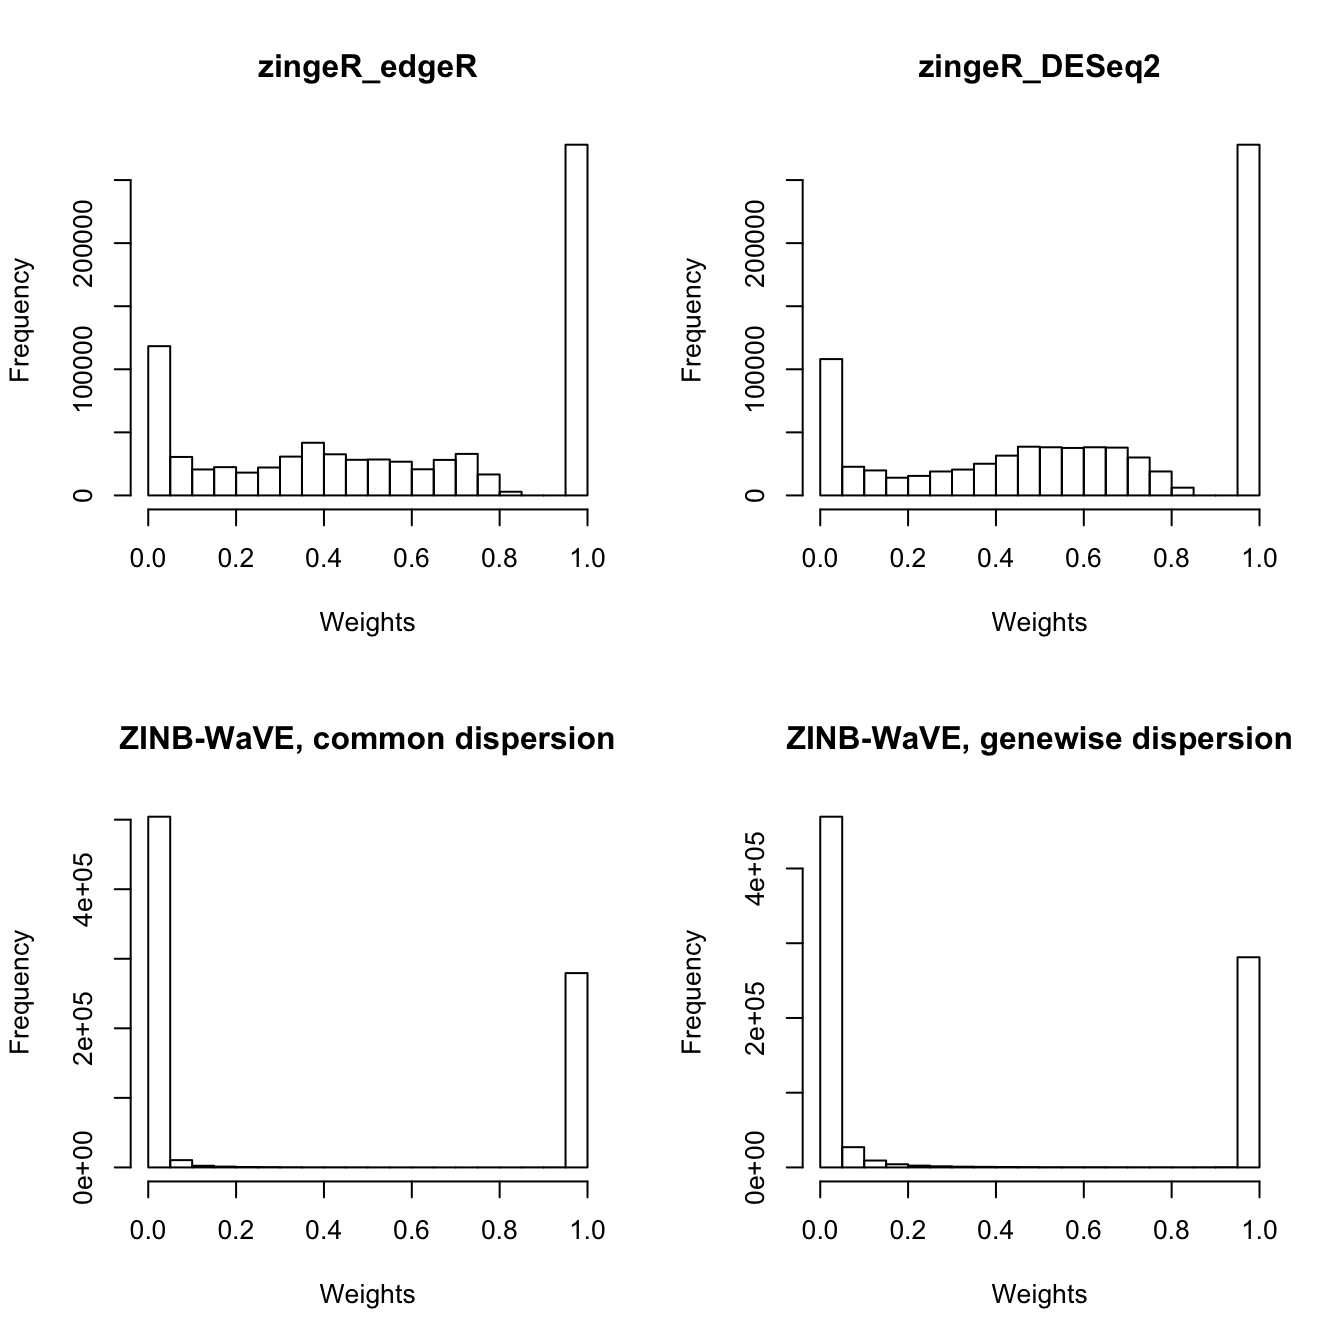
\includegraphics[keepaspectratio=true,scale=0.3]{islamWeightsFC2-1}
\end{center}
\caption{{\em Comparison of the distribution of the weights between zingeR and ZINB-WaVE.}}
\label{f:islamWeightsFC2}
\end{figure}


\begin{figure}[ht]
\begin{center}
\begin{tabular}{cccc}
\textbf{A} &
\includegraphics[keepaspectratio=true,scale=0.17,valign=t]{mocksBoxplot-1} &
\textbf{B} &
\includegraphics[keepaspectratio=true,scale=0.17,valign=t]{mocksPvalues-1} 
\end{tabular}
\end{center}
\caption{{\em ZINB-WaVE can control FDR.}}
\label{f:mocks}
\end{figure}

\begin{figure}[ht]
\begin{center}
\begin{tabular}{cccc}
\textbf{A} &
\includegraphics[keepaspectratio=true,scale=0.17,valign=t]{mocksEspilonFPR-1} &
\textbf{B} &
\includegraphics[keepaspectratio=true,scale=0.17,valign=t]{mocksEspilonPvalues-1} 
\end{tabular}
\end{center}
\caption{{\em Influence of regularization parameter on FPR and ditribution of pvalues}}
\label{f:mocksEpsilon}
\end{figure}


\begin{figure}[ht]
\begin{center}
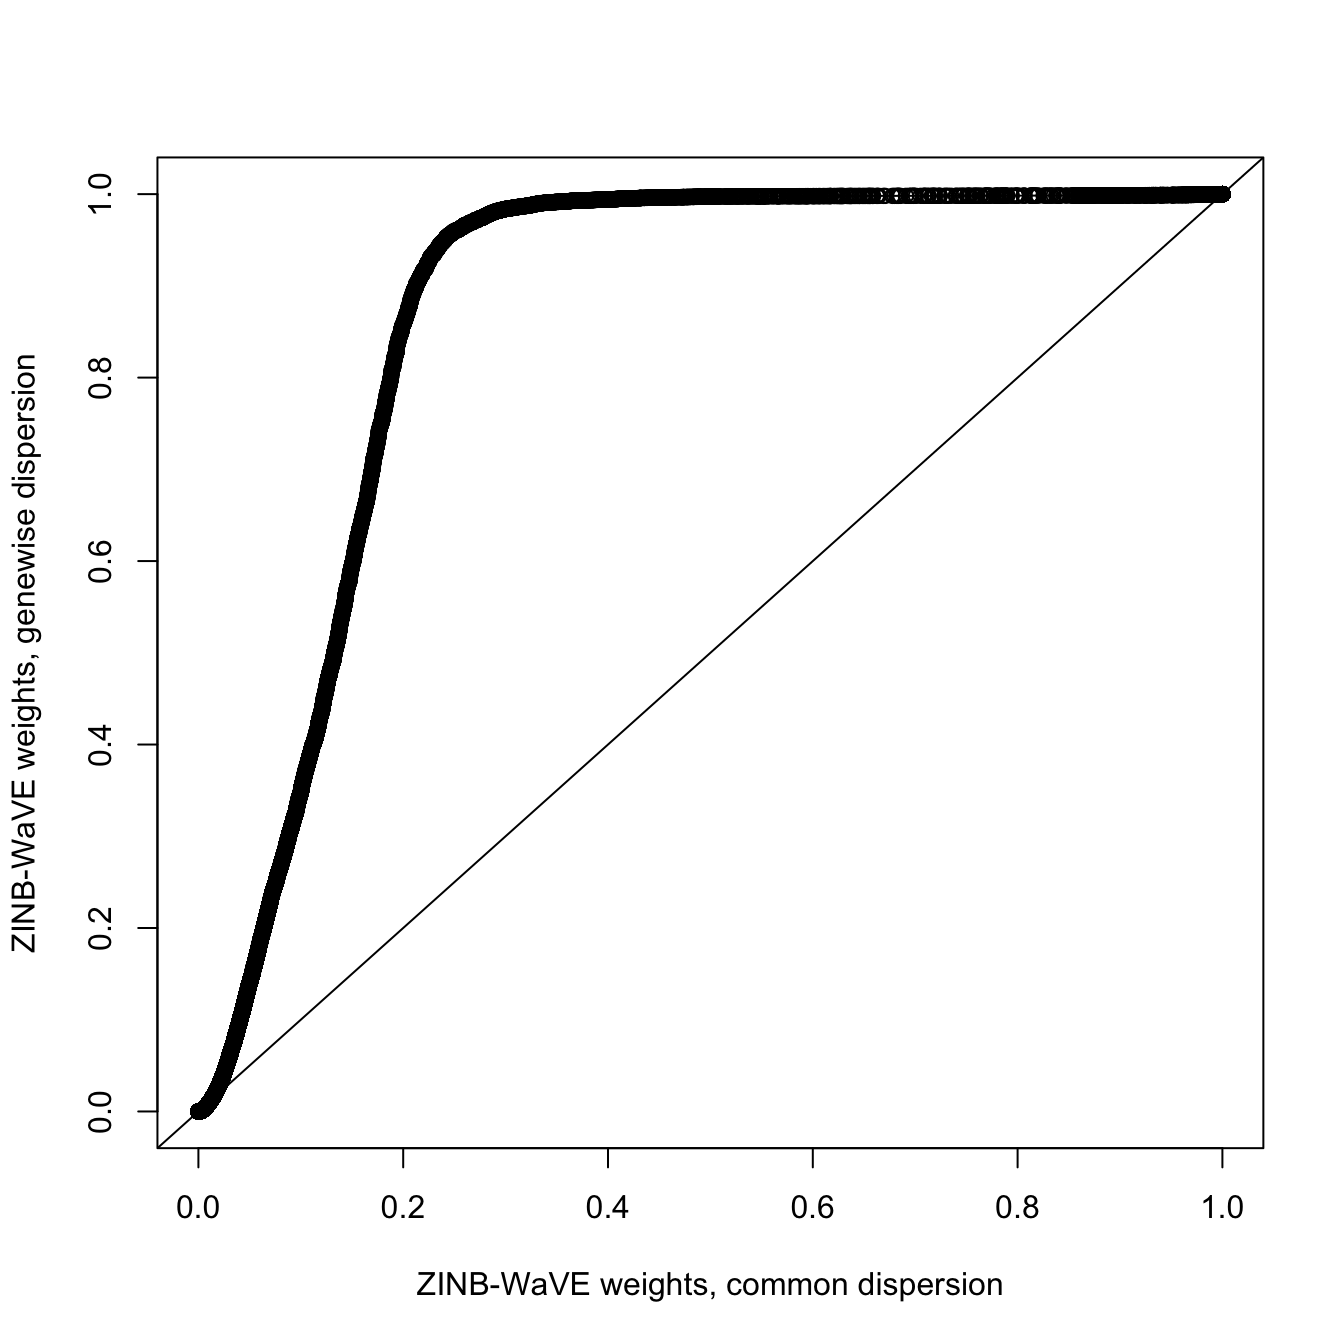
\includegraphics[keepaspectratio=true,scale=0.2]{qqplotFC2-1}
\end{center}
\caption{{\em QQplot of ZINB-WaVE weights for genewise and common dispersion.}}
\label{f:qqplotFC2}
\end{figure}

\section*{Methods}

\subsection*{ZINB-WaVE}

For any \(\pi\in[0,1]\), let \(f_{ZINB}( \cdot;\mu,\theta, \pi)\) be the probability mass function (PMF) of the zero-inflated negative binomial (ZINB) distribution given by:
\begin{equation}
f_{ZINB}(y;\mu,\theta, \pi) = \pi \delta_0(y) + (1-\pi) f_{NB}(y;\mu,\theta), \quad \forall y\in\mathbb{N},
\end{equation} 
where 
$f_{NB}(y;\mu,\theta)$ denotes the negative binomial (NB) PMF with mean $\mu$ and dispersion $\theta$ and \(\delta_0(\cdot)\) denotes the Dirac function. Here, \(\pi\) can be
interpreted as the probability of a droupout, i.e., that a zero is observed instead of the
actual count, resulting in an inflation of zeros compared to the NB distribution. 

Given \(n\) samples (typically, \(n\) single cells) and \(J\) features
(typically, \(J\) genes) that can be counted for each sample, let
\(Y_{ij}\) denote the count of feature \(j\) (for \(j=1,\ldots,J\)) for
sample \(i\) (\(i=1,\ldots,n\)). To account for various technical and
biological effects frequent in single-cell sequencing
technologies, we model \(Y_{ij}\) as a random variable following a ZINB
distribution with parameters \(\mu_{ij}\), \(\theta_{ij}\), and
\(\pi_{ij}\), and consider the following regression models for these parameters:
\begin{align}
\label{eq:model1}
\ln(\mu_{ij}) &= \left( X\beta_\mu + (V\gamma_\mu)^\top + W\alpha_\mu + O_\mu\right)_{ij}\,,\\
\label{eq:model2}
\text{logit}(\pi_{ij}) &= \left(X\beta_\pi + (V\gamma_\pi)^\top + W\alpha_\pi + O_\pi\right)_{ij} \,, \\
\label{eq:model3}
\ln(\theta_{ij}) &= \zeta_j \,.
\end{align}

Both the mean expression level ($\mu$) and the probability of dropouts ($\pi$) are modeled in terms of \textit{observed} sample-level and gene-level covariates ($X$ and $V$, respectively). In addition, we include a set of \textit{unobserved} sample-level covariates ($W$) that need to be inferred from the data. The matrix $X$ can include covariates that induce variation of interest, such as cell types, or covariates that induce unwanted variation, such as batch or quality control (QC) measures. It can also include a constant column of ones for an intercept that accounts for gene-specific differences in mean expression level or dropout rate. The matrix $V$ can also accommodate an intercept to account for cell-specific global effects, such as size factors representing differences in library sizes (i.e., total number of reads per sample). In addition, $V$ can include gene-level covariates, such as gene length or GC-content.\\ 

The model is fit using a penalized likelihood method. See \cite{Risso2017} for more details on the model and parameter estimation.

\subsection*{scRNA-seq data simulation}

The scRNA-seq simulation is based on the Islam mouse dataset \cite{Islam2011CharacterizationRNA-seq}, which compares 48 embryonic stem cells to 44 embryonic fibroblasts in mouse. We use the same simulation framework as the one described in \cite{VandenBerge2017ZingeR:Applications} and implemented in the zingeR package, where positive and zero counts are simulated separately using a Hurdle model.\\ 

Specifically, positive counts are simulated as follows. For each gene $j$, the mean expression level ($\lambda_j$) and dispersion ($\phi_j$) are estimated from a zero truncated negative binomial (ZTNB) distribution fit across all $n$ cells. The estimated parameters are then used to simulate positive counts for each cell $i$ and gene $j$ using a ZTNB with mean $\hat \mu_{ij} = \hat \lambda_{j} N_i$ and dispersion $\hat \phi_j$, where $N_i$ is the total number of reads for cell $i$ in a real dataset. \fp{Check. In zingeR paper, $\lambda{ij}$. Is it the same as $\lambda{j}$?}\\

Zero counts are simulated as follows. For each gene $j$, zero counts are simulated from a binomial distribution, where the parameter $p_j$ is estimated from a real dataset as
$$p_j = \frac{\sum_{i=1}^n p_{ij}}{n},$$
where $p_{ij}$ is estimated from a function depending on the average log count per million (CPM) of gene $j$ and the total number of reads for cell $i$ ($N_i$). See more details about the simulation framework in \cite{VandenBerge2017ZingeR:Applications}.

\subsection*{Case study}
Fletcher

\subsection*{Method comparison}
\begin{itemize}
  \item Bulk: edgeR, DESeq2, limma
  \item Single cell: MAST, zingeR-edgeR, zingeR-DESeq2, zingeR-limma
  \item Us: zinbwave-edgeR, zinbwave-DESeq2, zinbwave-limma with common and genewise dispersion
\end{itemize}

\subsection*{Implementation}
github repo, Rmd to reproduce the figures

\subsection*{Acknowledgements}
zingeR team

\subsection*{Grants}
\subsection*{Author contributions}

\pagebreak
\printbibliography
\appendix
\section*{Supplementary figures}

\begin{figure}[ht]
\begin{center}
\begin{tabular}{cccc}
\textbf{A} &
\includegraphics[keepaspectratio=true,scale=0.16,valign=t]{islamROCfc3-1} &
\textbf{B} &
\includegraphics[keepaspectratio=true,scale=0.16,valign=t]{islamPvaluesFC3-1} 
\end{tabular}
\end{center}
\caption{{\em Simulations from Islam dataset using zingeR simulation framework.} Fold change = 3, 80 cells, 10k genes. Panel (A) : ROC. Panel (B) Distr. of pval.}
\label{f:islamFC3}
\end{figure}

\end{document}
